\documentclass{article}
\usepackage{graphicx} % Required for inserting images
\usepackage{tabularx}
\usepackage{float}
\usepackage{longtable}
\usepackage[english,polish]{babel}
\usepackage{polski}
\usepackage[top=3cm, bottom=2cm, left = 3cm, right = 3cm]{geometry}
\usepackage[export]{adjustbox}

\title{Obliczenia Naukowe Lista 3}
\author{Bartłomiej Puchała}
\date{November 2023}

\begin{document}

\maketitle

\section{Zadanie 1}
\subsection{Opis problemu}
Problem polega na zaimplementowaniu funkcji rozwiązującej równanie $f(x) = 0$ metodą bisekcji. Metoda bisekcji jest jedną z metod rozwiązywania równań nieliniowych. Ogólną ideą tej metody jest zasada połowienia przedziałów. Chcąc zastosować tą metodę, należy przyjąć pewne założenia, tzn:
\begin{enumerate}
    \item Funkcja $f$ musi być funkcją ciągłą w \([a,b]\) - Ciągłość funkcji gwarantuje, iż jej wartości nie wykonują nagłych skoków i dla dowolnych dwóch wartości funkcji w tym przedziale znajdziemy wszystkie wartości pośrednie. 
    \item Funkcja musi zmieniać znak w zadanym przedziale \([a,b]\), tzn.
    $f(a)f(b) < 0$ - Ten warunek gwarantuje, że w przedziale \([a,b]\) istnieje taki argument $x_0$, dla którego $f(x_0) = 0$(Gwarancja istnienia przynajmniej jednego pierwiastka)
\end{enumerate}
Jeżeli te założenia są spełnione, to możliwe jest wyznaczanie środków przedziałów 
$$ c_n = \frac{1}{2}(a_n + b_n)$$  
Pierwiastki są znajdowane na podstawie kolejnych przybliżeń, należy więc określić dokładność, z jaką chcemy otrzymać pierwiastek funkcji oraz dokładność wyznaczania samej wartości funkcji $f(x)$, tzn. warunkami końca będą takie warunki:
\begin{enumerate}
    \item $|f(c_n)| \leq \epsilon $
    \item $|b_n - a_n| \leq \delta $
\end{enumerate}
Algorytm w każdym kroku dzieli przedział \([a,b]\) na 2 równe połowy $[a_n, c_n]$ oraz $[c_n, b_n]$. Algorytm przyjmuje za nowy przedział $[a, b]$ tą połówkę, dla której na krańcach przedziału funkcja $f(x)$ zmienia znak i kontynuuje wyznaczanie pierwiastka. Metoda ta jest zbieżna liniowo, wykładnik zbieżności $ \alpha = 1 $, metoda jest zbieżna globalnie.
\subsection{Rozwiązanie}
Ta funkcja znajduje się w module Functions
\begin{verbatim}
function mbisekcji(f::Function, a::Float64, b::Float64, delta::Float64, epsilon::Float64)::Int64
    err::Int
    it = 0
    u = f(a)
    v = f(b)
    e = b - a
    if(sign(u) == sign(v)) 
        err = 1
        return (0, 0, it, err)
    end

    while true
        e = e / 2
        c = a + e
        w = f(c)
        it += 1

        if(abs(e) < delta || abs(w) < epsilon)
            err = 0
            return (c, w, it, err)
        end

        if(sign(w) != sign(u))
            b = c
            v = w
        else 
            a = c
            u = w
        end
    end
end
\end{verbatim}
\section{Zadanie 2}
\subsection{Opis problemu}
Problem polega na zaimplementowaniu funkcji rozwiązującej równanie $f(x) = 0$ metodą Newtona. Metoda ta korzysta z funkcji liczących $f(x)$ oraz $f'(x)$. Aby możliwe było policzenie pierwiastka funkcji $f(x)$ w $[a,b]$ za pomocą tej metody, muszą zostać spełnione podane warunki:
\vspace{20pt}
\begin{enumerate}
    \item W przedziale $[a,b]$ pierwsza pochodna $f'(x) \neq 0$ - w obszarze poszukiwań pochodna funkcji nie powinna być równa $0$, w przeciwnym razie metoda może nie zbiegać
    \item Funkcja $f \in C^2[a,b]$, tzn. funkcja $f(x)$ jest dwukrotnie różniczkowalna na przedziale $[a,b]$, a ich drugie pochodne są ciągłe.
\end{enumerate}
Algorytm polega na wybraniu punktu początkowego $x_0$, od którego zacznie się poszukiwanie pierwiastka funkcji. Wybór tego punktu ma znaczenie, ponieważ przy źle wybranym punkcie startowym metoda może stać się rozbieżna. Następnie w każdej iteracji wyznaczamy za pomocą wzoru Newtona
$$ x_{n+1} = x_n - \frac{f(x_n)}{f'(x_n)} $$
kolejne przybliżenia pierwiastka, którymi są punkty przecięcia stycznej do wykresu funkcji $f(x)$ w punkcie $x_n$ z osią OX. Do wyznaczania kolejnego przybliżenia pierwiastka potrzebujemy tylko jednego punktu. Kolejne przybliżenia są wyznaczane, dopóki różnica pomiędzy dwoma kolejnymi wyznaczonymi pierwiastkami będzie zbyt mała lub wartość funkcji dla kolejnego $x_n$ przekroczy dokładność. Warunki końca metody prezentują się następująco:
\begin{enumerate}
    \item $|x_{n+1} - x_n| \leq \delta$
    \item $|f(x_{n+1})| \leq \epsilon$
\end{enumerate}
Graficzna interpretacja tej metody przedstawia się następująco:

\begin{figure}[H] 
\centering
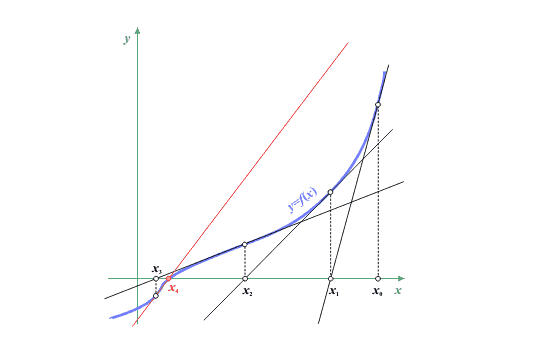
\includegraphics[width=0.9\textwidth, height=6cm]{Newton.png}
\caption{Graficzna interpretacja metody Newtona}
\label{Newton}
\end{figure}
Zaletą tej metody jest szybka zbieżność, wykładnik zbieżności $\alpha = 2$.
\subsection{Rozwiązanie}
Ta funkcja znajduje się w module Functions
\begin{verbatim}
function mstycznych(f::Function, pf::Function, x0::Float64, delta::Float64, epsilon::Float64, 
maxit::Int)
    v = f(x0)
    if abs(v) < epsilon
        return (x0, v, 0, 0) 
    end

    if abs(pf(x0)) < epsilon
        return (0, 0, 0, 2) # pochodna bliska zeru
    end

    for k in 1:maxit
        x1 = x0 - v / pf(x0)
        v = f(x1)
        if(abs(v) < epsilon || abs(x1 - x0) < delta)
            return (x1, v, k, 0)
        end
        x0 = x1
    end
    # nie osiągnięto wymaganej dokładności w maxit iteracji
    return (0, 0, 0, 1)
end
\end{verbatim}

\section{Zadanie 3}
\subsection{Opis problemu}
Problem polega na zaimplementowaniu funkcji rozwiązującej równanie $f(x) = 0$ metodą siecznych. Metoda ta jest podobna do metody Newtona, ale do jej wykonania niepotrzebne jest liczenie pochodnej funkcji $f'(x)$, jest ona aproksymowana przez iloraz różnicowy, tzn:
$$ f'(x_n) \approx \frac{f(x_n) - f(x_{n-1})}{x_n - x_{n-1}} $$
Aby możliwe było policzenie pierwiastka funkcji $f(x)$ w $[a, b]$ za pomoca tej metody,
musza zostać spelnione podane warunki:
\begin{enumerate}
    \item W przedziale $[a,b]$ pierwsza pochodna $f'(x) \neq 0$ - ten warunek gwarantuje, iż sieczna nie będzie równoległa do osi OX, co uniemożliwiłoby wyznaczenie jej punktu przecięcia z tą osią
    \item Funkcja $f \in C^2[a,b]$, tzn. funkcja $f(x)$ jest dwukrotnie różniczkowalna na przedziale $[a,b]$, a ich drugie pochodne są ciągłe.
\end{enumerate}
Algorytm polega na iteracyjnym obliczeniu kolejnych przybliżeń pierwiastka, wykorzystując dwa poprzednio wyznaczone przybliżenia pierwiastka za pomocą wzoru:
$$ x_{n+1} = x_n - \frac{x_n - x_{n-1}}{f(x_n) - f(x_{n-1})}f(x_n) $$
Wzór ten jest analogiczny co do wzoru Newtona, lecz zamiast wartości pochodnej funkcji $f(x)$ do wzoru podstawiamy jej aproksymację. Chcąc otrzymać kolejne przybliżenie pierwiastka, konstruujemy sieczną do wykresu funkcji $f(x)$ przecinającą $f(x)$ w punktach $x_n$ oraz $x_{n-1}$. Przecięcie tej siecznej z osią OX będzie kolejnym przybliżeniem pierwiastka. Warunkami końca tej metody są:
\begin{enumerate}
    \item $|x_{n+1} - x_n| \leq \delta$
    \item $|f(x_{n+1})| \leq \epsilon$
\end{enumerate}
Metoda ta ma współczynnik zbieżności $\alpha = (1 + \sqrt{5})/2$, jej graficzna interpretacja prezentuje się następująco:

\begin{figure}[H] 
\centering
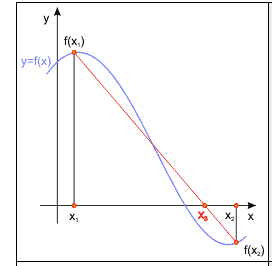
\includegraphics[width=0.85\textwidth, height=6cm]{Sieczne.png}
\caption{Graficzna interpretacja metody siecznych}
\label{Sieczne}
\end{figure}
\newpage
\subsection{Rozwiązanie}
Ta funkcja znajduje się w module Functions
\begin{verbatim}
function msiecznych(f::Function, x0::Float64, x1::Float64, delta::Float64, epsilon::Float64, 
maxit::Int)
    fa = f(x0)
    fb = f(x1)
    for k in 1:maxit
        if(abs(fa) > abs(fb))
            tmp = x0
            tmp_f = fa
            x0 = x1
            x1 = tmp
            fa = fb
            fb = tmp_f
        end
        s = (x1 - x0) / (fb - fa)
        x1 = x0
        fb = fa
        x0 = x0 - (fa * s)
        fa = f(x0)
        if(abs(x1 - x0) < delta || abs(fa) < epsilon)
            return (x0, fa, k, 0)
        end
    end
    return (0, 0, 0, 1)
end
\end{verbatim}

\section{Zadanie 4}
\subsection{Opis problemu}
Problem polega na zastosowaniu metod rozwiązywania równań do wyznaczenia pierwiastka równania:
$$ sin(x) - (\frac{1}{2}x)^2 = 0$$
Należy zastosować:
\begin{enumerate}
    \item Metodę bisekcji z przedziałem początkowym $[1.5, 2]$ i $\delta = \frac{1}{2}10^{-5}, \epsilon = \frac{1}{2}10^{-5}$.
    \item Metodę Newtona z przybliżeniem początkowym $x_0 = 1.5$ i $\delta = \frac{1}{2}10^{-5}, \epsilon = \frac{1}{2}10^{-5}$.
    \item Metodę siecznych z przybliżeniami początkowymi $x_0 = 1$ i $x_1 = 2$ i $\delta = \frac{1}{2}10^{-5}, \epsilon = \frac{1}{2}10^{-5}$.
\end{enumerate}
\subsection{Rozwiązanie}
\begin{verbatim}
include("./Functions.jl")
using .Functions

function f(x)
    return sin(x) - (1/4)x^2
end

function pf(x)
    return cos(x) - (1/2)x
end

a = 1.5
b = 2.0
x0 = 1.5
delta = (1/2) * 10^(-5)
epsilon = (1/2) * 10^(-5)
r, v, it, err = Functions.mbisekcji(f, a, b, delta, epsilon)
println("Pierwiastek to $r, wartość funkcji $v, liczba iteracji: $it, znak błędu: $err")

r, v, it, err = Functions.mstycznych(f, pf, x0, delta, epsilon, 10)
println("Pierwiastek to $r, wartość funkcji $v, liczba iteracji: $it, znak błędu: $err")

x0 = 1.0
x1 = 2.0
r, v, it, err = Functions.msiecznych(f, x0, x1, delta, epsilon, 10)
println("Pierwiastek to $r, wartość funkcji $v, liczba iteracji: $it, znak błędu: $err")
\end{verbatim}
\subsection{Wyniki i interpretacja}
\vspace{10pt}
\setlength{\tabcolsep}{2pt}
\renewcommand{\arraystretch}{1.6}
\newcolumntype{Y}{>{\raggedright\arraybackslash}X}
\begin{tabularx}{\textwidth}{|l|Y|Y|l|}
\hline
Algorytm & x & f(x) & Iteracje \\
\hline
Bisekcja & 1.9337539672851562 & -2.7027680138402843e-7 & 16 \\
\hline
Newtona & 1.933753779789742 & -2.2423316314856834e-8 & 4 \\
\hline
Siecznych & 1.933753644474301 & 1.564525129449379e-7 & 4 \\
\hline
\end{tabularx}
\vspace{15pt}

Ta funkcja oprócz miejsca zerowego $x_0 = 0$ posiada miejsce zerowe $f(x) = 0$ dla $x \approx 1.93375$, więc każda metoda zwróciła poprawny wynik, różnica w liczbie iteracji dla danej metody wynika z faktu, że każda z metod ma różny współczynnik zbieżności $\alpha$.
\subsection{Wnioski}
Mając dobrze zadaną funkcję każda z metod potrafi zwrócić poprawny wynik z zadaną dokładnością, poszczególne metody różnią się tylko liczbą iteracji.

\section{Zadanie 5}
\subsection{Opis problemu}
Problem polega na znalezieniu metodą bisekcji wartości zmiennej $x$, dla której przecinają się wykresy funkcji $y = 3x$ i $y = e^x$ z dokładnością obliczeń $\delta = 10^{-4}, \epsilon = 10^{-4}$.
\subsection{Rozwiązanie}
Aby znaleźć wartości zmiennej $x$, dla których przecinają się wykresy funkcji $f(x)$ należy rozwiązać równanie
$$ e^x = 3x $$
co po przekształceniu daje postać 
$$ e^x - 3x = 0 $$
Wykres funkcji $f(x) = e^x - 3x$ przedstawia się następująco:

\begin{figure}[H] 
\centering
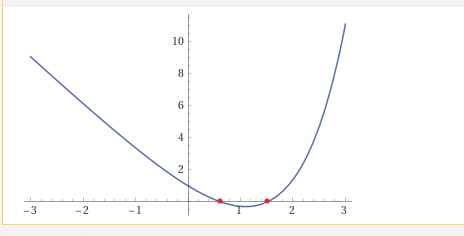
\includegraphics[width=0.85\textwidth, height=6.5cm]{e_x.png}
\caption{f(x) = e^x - 3x}
\label{Zadanie 5}
\end{figure}
\vspace{10pt}
Należy więc się spodziewać się pierwiastków w przedziałach $[0,1]$ i $[1,2]$, dlatego wybrałem te dwa przedziały jako parametry do metody bisekcji.
\begin{verbatim}
include("./Functions.jl")
using .Functions

delta = 10^(-4)
epsilon = 10^(-4)
e_value = Base.MathConstants.e
println(e_value)

function f(x)
    return e_value^(x) - 3x
end

# e^x = 3x
# e^x - 3x = 0
a = 1.0
b = 2.0
r, v, it, err = Functions.mbisekcji(f, a, b, delta, epsilon)
println("Pierwiastek to $r, wartość funkcji $v, liczba iteracji: $it, znak błędu: $err")
\end{verbatim}
\subsection{Wyniki i interpretacja}
\vspace{10pt}
\setlength{\tabcolsep}{2pt}
\renewcommand{\arraystretch}{1.6}
\newcolumntype{Y}{>{\raggedright\arraybackslash}X}
\begin{tabularx}{\textwidth}{|l|Y|Y|l|}
\hline
Przedział & x & f(x) & Iteracje \\
\hline
$[0,1]$ & 0.619140625 & -9.066320343276146e-5 & 9 \\
\hline
$[1,2]$ & 1.5120849609375 & -7.618578602741621e-5 & 13 \\
\hline
\end{tabularx}
\vspace{15pt}
\subsection{Wnioski}
Dla odpowiednio dobranych startowych przedziałów za pomocą metody bisekcji można w poprawny sposób wyznaczyć miejsca zerowe funkcji.
\section{Zadanie 6}
\subsection{Opis problemu}
Problem polega na znalezieniu miejsc zerowych funkcji $f_1(x) = e^{1 - x} - 1 $ oraz $f_2(x) = xe^{-x}$ za pomocą metody bisekcji, Newtona i siecznych z wymaganą dokładnością $\delta = 10^{-5}$ oraz $\epsilon = 10^{-5}$
\subsection{Rozwiązanie}
\begin{verbatim}
include("./Functions.jl")
using .Functions

delta = 10^(-5)
epsilon = 10^(-5)
e = Base.MathConstants.e

function f1(x)
    return e^(1 - x) - 1
end

function pf1(x)
    return -e^(1 - x)
end

function f2(x)
    return x*e^(-x)
end

function pf2(x)
    return -e^(-x)*(x - 1)
end

a = -1.5
b = 0.5
r, v, it, err = Functions.mbisekcji(f2, a, b, delta, epsilon)
println("Pierwiastek to $r, wartość funkcji $v, liczba iteracji: $it, znak błędu: $err")
x0 = -1.5
r, v, it, err = Functions.mstycznych(f2, pf2, x0, delta, epsilon, 10)
println("Pierwiastek to $r, wartość funkcji $v, liczba iteracji: $it, znak błędu: $err")
x0 = -1.5
x1 = 0.5
r, v, it, err = Functions.msiecznych(f2, x0, x1, delta, epsilon, 10)
println("Pierwiastek to $r, wartość funkcji $v, liczba iteracji: $it, znak błędu: $err")
\end{verbatim}
Dla podanych metod jako przedziały przyjąłem następujące dane:

\setlength{\tabcolsep}{2pt}
\renewcommand{\arraystretch}{1.6}
\newcolumntype{Y}{>{\raggedright\arraybackslash}X}
\begin{tabularx}{\textwidth}{|l|l|X|}
\hline
Metoda & funkcja & params \\
\hline
Bisekcja & f1 & $a=0.5, b = 2.0$ \\
\hline
Bisekcja & f2 & $a=-1.5, b = 0.5$ \\
\hline
Newton & f1 & $x_0 = 0.5$ \\
\hline
Newton & f2 & $x_0 = -1.5$ \\
\hline
Sieczne & f1 & $x_0 = 0.5, x_1 = 1.5$ \\
\hline
Sieczne & f2 & $x_0 = -1.5, x_1 = 0.5$ \\
\hline
\end{tabularx}
\vspace{15pt}
\subsection{Wyniki i interpretacja}
\vspace{10pt}
Wyniki dla funkcji $f_1(x) = e^{1 - x} - 1$ \\

\vspace{8pt}
\setlength{\tabcolsep}{2pt}
\renewcommand{\arraystretch}{1.6}
\newcolumntype{Y}{>{\raggedright\arraybackslash}X}
\begin{tabularx}{\textwidth}{|l|Y|Y|l|}
\hline
Algorytm & x & f(x) & Iteracje \\
\hline
Bisekcja & 0.9999923706054688 & 7.629423635080457e-6 & 16 \\
\hline
Newton & 0.9999999998878352 & 1.1216494399945987e-10 & 4 \\
\hline
Sieczne & 0.9999999624498374 & 3.755016342310569e-8 & 5 \\
\hline
\end{tabularx}
\vspace{15pt}

Wyniki dla funkcji $f_2(x) = xe^{-x}$ \\

\vspace{7pt}
\setlength{\tabcolsep}{2pt}
\renewcommand{\arraystretch}{1.6}
\newcolumntype{Y}{>{\raggedright\arraybackslash}X}
\begin{tabularx}{\textwidth}{|l|Y|Y|l|}
\hline
Algorytm & x & f(x) & Iteracje \\
\hline
Bisekcja & 0.0 & 0.0 & 2 \\
\hline
Newton & -4.179471505818752e-8 & -4.179471680498576e-8 & 6 \\
\hline
Sieczne & 1.7791419742860986e-8 & 1.779141942632637e-8 & 8 \\
\hline
\end{tabularx}
\vspace{10pt}

Jak widać metoda siecznych potrzebowała więcej iteracji od metody Newtona, co wynika z różnego współczynnika zbieżności $\alpha$. Dla dobrze wybranych parametrów metoda Bisekcji potrafi w szybszym czasie zwrócić pierwiastek funkcji $f(x)$. Jeżeli chodzi o testy dla metody Newtona dla $x_0 \in (1,\infty)$ dla funkcji $f_1$, to wraz ze wzrostem wartości punktu startowego $x_0$ rośnie liczba iteracji metody, aby dla $x_0 = 7$ osiągnąć aż 401 iteracji, a dla większych punktów startowych metoda nie osiąga wymaganej dokładności w maxit iteracji. Dla metody Newtona i funkcji $f_2$ i punktu $x_0 > 1$ otrzymuję niepoprawne wyniki, co jest spowodowane że $lim_{x -> \infty}{f_2'(x)} = 0$, więc wartości są coraz bardziej niedokładne w arytmetyce. Dla $x_0 = 1$ i funkcji $f_2$ nie można wybrać tego punktu $x_0$, ponieważ $f_2'(1) = 0$, co spowoduje, że styczna będzie równoległa do osi OX dzięki czemu niemożliwe będzie wyznaczenie punktu przecięcia i kolejnych przybliżeń pierwiastka.
\newpage

\subsection{Wnioski}
Źle dobrane parametry początkowe mogą spowodować błędy w otrzymywanych wynikach. W przypadku implementowania algorytmów poszukujących pierwiastków danych równań, warto zastosować różne metody do różnych celów, np. metodę Bisekcji do ograniczenia przedziału do przedziału, w którym blisko znajduje się miejsce zerowe funkcji, aby potem zastosować metodę siecznych albo Newtona, aby w niewielkiej liczbie iteracji otrzymać poprawny wynik.
\end{document}
